\chapter{Theory}

\section{A brief introduction to statistical mechanics}
The discussion in this section is mostly based on the ``Introduction to Computational Chemistry'' textbook written by Jensen~\citep{jensenIntroductionComputationalChemistry2017}, ``Statistical Mechanics: Theory and Molecular Simulation'' by Tuckermann~\citep{tuckermanStatisticalMechanicsTheory2023}, and ``Understanding Molecular Simulation: From Algorithms to Applications'' by Frenkel and Smit~\citep{frenkelUnderstandingMolecularSimulation2002} unless stated otherwise.



\subsection{Partition functions}
The development of the field of statistical mechanics has been crucial for the computational chemistry community, as it enables the connection between the jigglings and wigglings of atoms and the properties of much larger systems such as liquids and solids.

Let us begin with the most fundamental concept: the partition function. The partition function is akin to a Swiss army knife in statistical mechanics, meaning it is a versatile tool that makes the connection between microscopic and macroscopic properties in thermodynamics possible. In the simplest case of a single molecule, the partition function $q$ takes the following form:

\begin{equation}
    q = \sum_{i = \text{levels}}^{\infty} g_i e^{-\epsilon_i/kT}
\end{equation}

Here, it is expressed as a sum over all energy levels $\epsilon_i$ of a molecule (or particle), multiplied by a degeneracy factor $g_i$ in cases where multiple levels have the same energy. The term $kT$ represents the Boltzmann factor.

Moving on to a more complex scenario in which the partition function describes multiple molecules, we arrive at the partition function $Q$ for non-interacting particles, such as those in an ideal gas:

\begin{equation}
    \label{eq:Q_noninteracting}
    Q = q^N \; \text{(different particles)} \quad Q = \frac{q^N}{N!} \; \text{(identical particles)}
\end{equation}

Here, $N$ denotes the total number of particles. However, one could argue that if we wish to describe a real system such as bulk water, we must account for interactions between molecules. Consequently, Equation~\ref{eq:Q_noninteracting} must be rewritten:

\begin{equation}
    Q = \sum_{i}^{\infty} e^{-E_i/kT}
\end{equation}

In this case, the partition function $Q$ includes contributions from all possible energy states $E_i$ of the system.

Although the concept of the partition function might initially appear abstract, it can be clarified by expressing it in a different form, namely, within the context of the \ac{rrho} approximation, where the electronic, vibrational, and rotational degrees of freedom can be separated. For a single molecule case it would look like:

\begin{equation}
    q_{\text{tot}} = q_{\text{trans}} \times q_{\text{rot}} \times q_{\text{vib}} \times q_{\text{elec}}
\end{equation}

Let us now examine each contribution in more detail. From this point onward we will consider polyatomic molecules in the formulation of the partition functions, unless stated otherwise.

The translational partition function $q_\text{trans}$ can be derived from the energy expression for a particle in a one-dimensional box and is given by:

\begin{equation}
    q_{\text{trans}} = \left(\frac{2\pi MkT}{h^2}\right)^{3/2} V
\end{equation}

Here, $M$ is the total molecular mass, and $V$ is the volume. Turning to the rotational partition function $q_\text{rot}$, it can be derived from the Schr\"odinger equation for a diatomic "rigid rotor" and has the following form:

\begin{equation}
    q_{\text{rot}} = \frac{8\pi^2IkT}{h^2\sigma}
\end{equation}

In this expression, $I$ denotes the moment of inertia, and $\sigma$ represents the symmetry factor, i.e. the order of the rotational subgroup within the molecular point group. For polyatomic molecules, writing an exact expression is more complex, but an approximate form can be used:

\begin{equation}
    q_{\text{rot}} = \frac{\sqrt{\pi}}{\sigma}\left(\frac{8\pi^2kT}{h^2}\right)^{3/2} \sqrt{I_1I_2I_3}
\end{equation}

For the vibrational partition function $q_\text{vib}$, it is expressed as a product over the various vibrational modes of a molecule, each with frequency $\nu_i$:

\begin{equation}
    q_{\text{vib}} = \prod_{i} \frac{e^{-h\nu_i/2kT}}{1-e^{-h\nu_i/kT}}
\end{equation}

Lastly, the electronic partition function $q_\text{elec}$ is given as a sum over all electronic states of a molecule, from the ground state to all excited states. However, since the energy difference between the ground state and higher states is usually much greater than $kT$ at ambient temperatures, the function can typically be approximated by considering only the ground state:

\begin{equation}
    q_{\text{elec}} = \sum_{i=0}^{\infty} g_i e^{-\epsilon_i/kT} \approx g_0 e^{-\epsilon_0/kT}
\end{equation}

This contribution can thus be calculated by solving the electronic Schr\"odinger equation. 



\subsection{Macroscopic properties and thermodynamic functions}

Once the partition function is determined, it provides a direct means of evaluating macroscopic properties. For instance, the internal energy $U$ and the Helmholtz free energy $A$ can be calculated from the partition function $Q$:

\begin{align}
    U &= kT^2 \left(\frac{\partial \ln Q}{\partial T}\right)_V \\
    A &= -kT\ln Q
\end{align}

In addition, other macroscopic properties, such as pressure $P$ and the heat capacity at constant volume $C_V$, can also be expressed in terms of the partition function:

\begin{align}
    P &= -\left(\frac{\partial A}{\partial V}\right)_T = kT\left(\frac{\partial \ln Q}{\partial V}\right)_T \\
    C_V &= \left(\frac{\partial U}{\partial T}\right)_V = 2kT\left(\frac{\partial \ln Q}{\partial T}\right)_V + kT^2\left(\frac{\partial^2 \ln Q}{\partial T^2}\right)_V
\end{align}

Turning to thermodynamic functions, namely enthalpy $H$, entropy $S$, and Gibbs free energy $G$, these can also be derived from the partition function $Q$:

\begin{align}
    H &= U + PV = kT^2\left(\frac{\partial \ln Q}{\partial T}\right)_V + kTV\left(\frac{\partial \ln Q}{\partial V}\right)_T \\
    S &= \frac{U-A}{T} = kT\left(\frac{\partial \ln Q}{\partial T}\right)_V + k\ln Q \\
    G &= H - TS = kTV\left(\frac{\partial \ln Q}{\partial V}\right)_T - kT\ln Q
\end{align}

This connection between macroscopic observables, thermodynamic functions, and the partition function once again highlights its fundamental importance in statistical thermodynamics.



\subsection{The canonical ensemble}
Having established a method to calculate the macroscopic properties of a system we implicitly relied on averaging over a large enough number of states. Therefore one may naturally ask: how can we sample enough configurations to apply the equations described in the previous section under conditions that resemble those in experiments? One such answer is the canonical ensemble.

The canonical ensemble describes a system at constant temperature $T$, fixed volume $V$, and a fixed number of particles $N$ (\acs{nvt}). In this ensemble, the system is in contact with a heat bath, which makes it particularly relevant to most molecular simulations that are describing the experimental conditions, where the temperature is externally controlled while the internal energy of the system is allowed to fluctuate.

Since the energy fluctuates in the canonical ensemble, a logical step is to estimate the magnitude of these fluctuations:

\begin{equation}
    \frac{\Delta E}{E} \sim \frac{\sqrt{N}}{N} \sim \frac{1}{\sqrt{N}}
\end{equation}

Here, $N$ denotes the number of particles, and thus for sufficiently large systems, the relative energy fluctuations become negligible.

The use of the canonical ensemble implicitly assumes that the system is ergodic, meaning that time averages obtained from simulation trajectories are equivalent to ensemble averages over the Boltzmann distribution. This assumption is, for instance, central to molecular dynamics simulations where the canonical ensemble can be sampled.

\subsection{Classical forcefields and molecular dynamics}

\subsection{Enhanced sampling techniques}

\begin{equation}
V_{\text{G}}(S(x), t) = w \sum_{t' = \tau_{\text{G}}, 2\tau_{\text{G}}, \ldots}^{t' < t} \exp\left(-\frac{(S(x) - s(t'))^2}{2\delta s^2}\right)
\label{eq:biasing_potential}
\end{equation}

\begin{equation}
\label{eq:free_energy_from_metadynamics}
\lim_{t \to \infty} V_G(s,t) \sim -F(s)
\end{equation}

\begin{equation}
V(s, t) = \Delta T \ln\left(1 + \frac{\omega N(s, t)}{\Delta T}\right)
\label{eq:history_dependant_potential}
\end{equation}

\begin{equation}
\label{eq:hill_deposition_rate}
\dot{V}(s,t) = \frac{\omega \Delta T \delta_{s,s(t)}}{\Delta T + \omega N(s,t)} 
= \omega e^{-[V(s,t)/\Delta T]} \delta_{s,s(t)}
\end{equation}

\begin{equation}
w = \omega e^{-[V(s,t)/\Delta T]} \tau_{\text{G}}
\label{eq:hill_height}
\end{equation}

\begin{equation}
\label{eq:free_energy_surface_reconstruction}
\tilde{F}(s,t) = -\frac{T + \Delta T}{\Delta T} V(s,t) 
= -(T + \Delta T) \ln\left(1 + \frac{\omega N(s,t)}{\Delta T} \right)
\end{equation}

\begin{figure}[htbp]
    \centering
    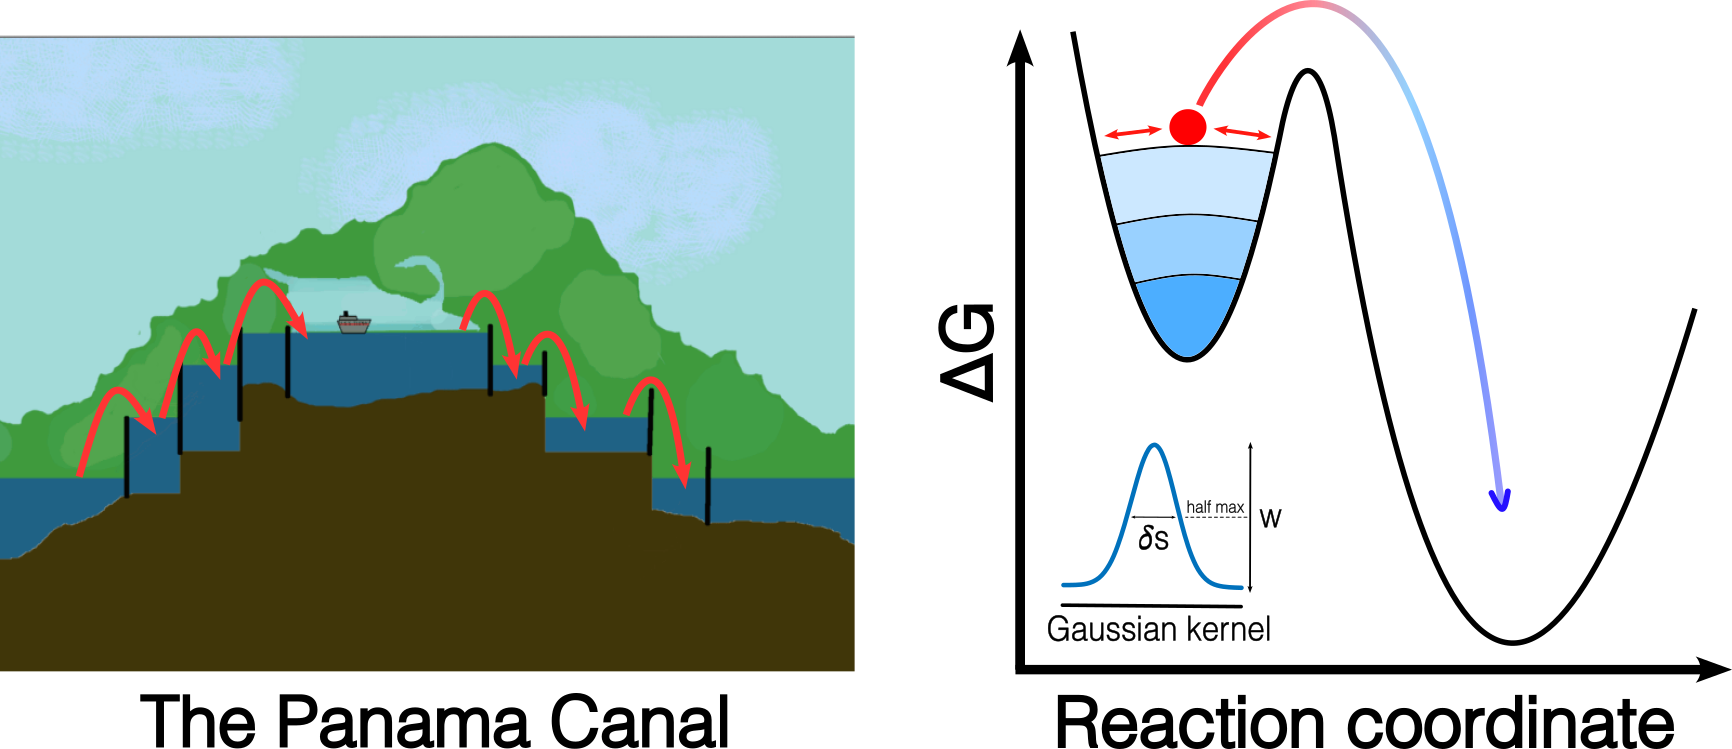
\includegraphics[width=0.8\textwidth]{Figures/2_Theory/theory_metadynamics.png}
    \caption{Metadynamics. The Panama Canal cartoon reproduced from~\citep{HowPanamaCanal}.}
    \label{fig:metadynamics}
\end{figure}



\section{Transition state theory}



\section{Density functional theory}

\subsection{The Kohn-Sham approach}

\subsection{Generalised gradient approximation and PBE functional}

\subsection{\textit{Ab initio} molecular dynamics and GPW method}



\section{Extended tight binding}



\section{Neural network potentials}

\subsection{Message passing graph neural networks}

\subsection{Invariance and equivariance}

\subsection{Equivariant neural network potentials}